\begin{frame}
    \frametitle{Kalman Filter}
    \note{information taken from https://youtu.be/PiCC-SxWlH8}
   
    \begin{itemize}
    \item It is a Bayes Filter
    \item Everything is Gaussian
    \begin{equation*}
    p(x)=\det(2\pi\covariance)^{\frac{1}{2}} \exp\left(-\dfrac{1}{2} (x - \mu )^{\top} \inverse{\covariance} (x - \mu ) \right)
    \end{equation*}
   
    \item Optimal solutions for linear models and Gaussian distributions.
    \end{itemize}
   
    \begin{figure}[!h]
    \centering
    \subfloat[\scriptsize Gaussian Distribution in 1D]
    {
    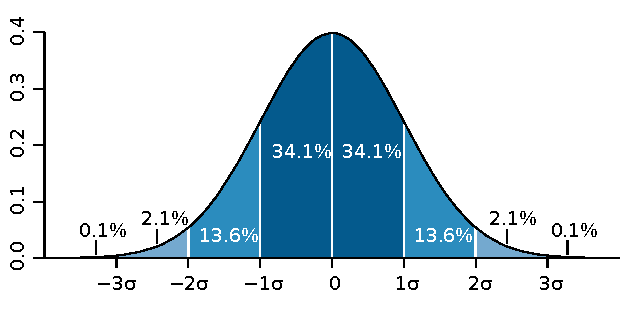
\includegraphics[width=0.3\columnwidth]{./images/standard_deviation_diagram.pdf}
    }
    \subfloat[\footnotesize 2D Gaussian Distribution]
    {
    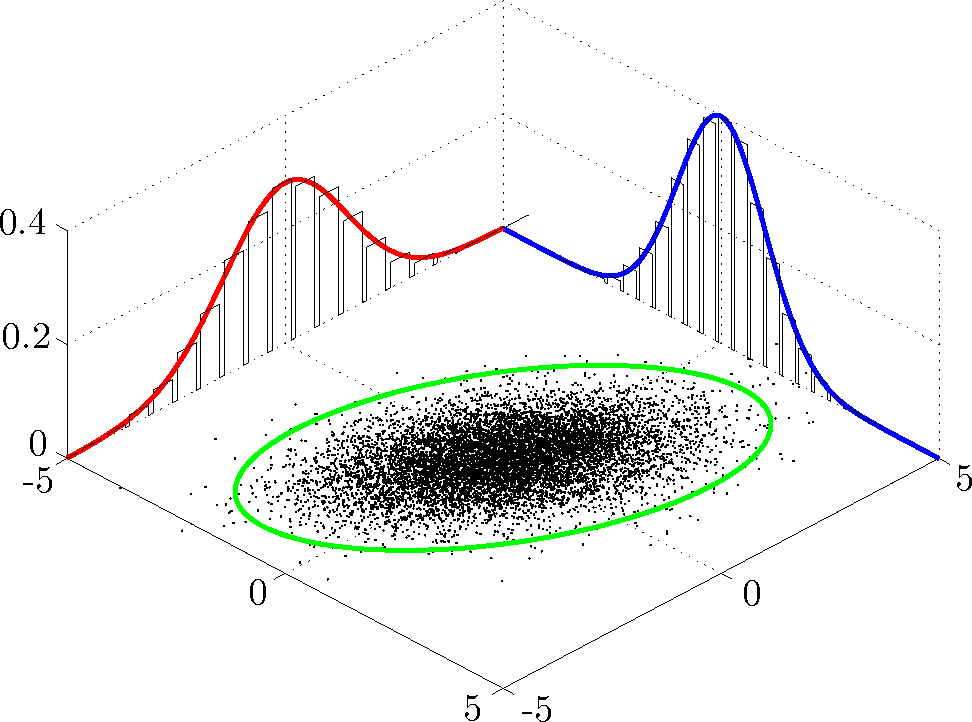
\includegraphics[width=0.3\columnwidth]{./images/multivariate_normal_sample.pdf}
    }
    \subfloat[\footnotesize 3D Gaussian Distribution]
    {
    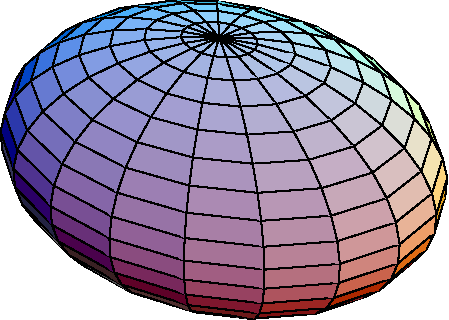
\includegraphics[width=0.25\columnwidth]{./images/ellipsoid.pdf}
    }
    \end{figure}
   \end{frame}
   
   
   \begin{frame}
    \frametitle{Kalman Filter Assumptions}
   \note{Information extracted from https://youtu.be/PiCC-SxWlH8}
   \note{Information extracted from https://www.youtube.com/watch?v=E-6paM\_Iwfc\&t=3442s}
   \small
   \begin{itemize}
   \item Noise and Gaussian Distributions
   \item Linear Motion and Observation Models
   \end{itemize}
   
   \begin{align*}
   \state_{t} &= \stateEvolutionMatrix_{t} \state_{t-1} + B_{t}\controlCommand_{t} + \motionModelNoise_{t}\\
   \observation_{t} &= C_{t} \state_{t} + \measurementModelNoise_{t}
   \end{align*}
   
   \begin{description}
   \item[$\stateEvolutionMatrix_{t}$] Matrix $(n \times n)$ describing how the state evolves from $t-1$ to $t$ without control commands or noise.
   
   \item[$B_{t}$] Matrix $(n \times l)$ describing how the control $\controlCommand_{t}$ changes the state from $t-1$ to $t$.
   
   \item[$C_{t}$] Matrix $(k \times n)$ describing how to map the state $\state_{t}$ to an observation $\observation_{t}$.
   
   \item[$\motionModelNoise_{t}$] Random variable representing the Gaussian noise of the motion model, assumed to be independent and normally distributed with mean zero and covariance $\motionParametersCovariance_{t}$.
   
   \item[$\measurementModelNoise_{t}$] Random variable representing the Gaussian noise of the {\bf observation model}, assumed to be independent and normally distributed with zero mean and covariance $\observationModelCovariance_{t}$.
   
   \end{description}
   
   \note{Kalman Filter requires that the noises be Gaussian and that the state result from a linear combination.}
   
   \note{Differential drive and Ackerman motion models are NOT linear models}
   \note{Observation models of a laser or a camera are also nonlinear.}
   \end{frame}
   
   \begin{frame}
   \frametitle{1D Kalman Filter}
   \note{Information taken from https://youtu.be/E-6paM_Iwfc}
   
   \begin{figure}[!h]
   \centering
   \subfloat[Initial Prediction]
   {
   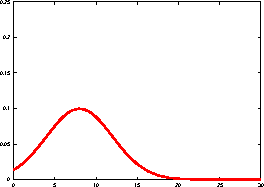
\includegraphics[width=0.3\columnwidth]{./images/kalman_filter_initial_prediction.pdf}
   }
   \subfloat[Measurement]
   { 
   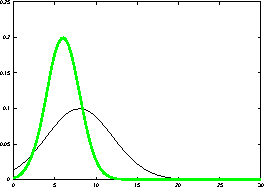
\includegraphics[width=0.3\columnwidth]{./images/kalman_filter_first_measurement.pdf}
    }
    \subfloat[Correction]
    {
    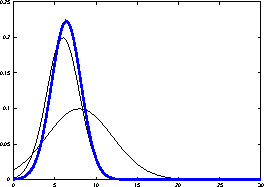
\includegraphics[width=0.3\columnwidth]{./images/kalman_filter_first_correction.pdf}
    }
    \end{figure}
   
   \end{frame}
   
   \begin{frame}
    \frametitle{1D Kalman Filter}
    \note{information taken from https://youtu.be/E-6paM_Iwfc}
   
    \begin{figure}[!h]
    \centering
    \subfloat[Motion Prediction]
    {
    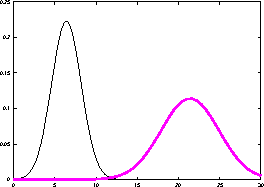
\includegraphics[width=0.3\columnwidth]{./images/kalman_filter_motion_prediction.pdf}
    }
    \subfloat[Second Measurement]
    {
    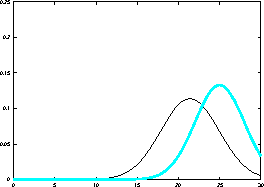
\includegraphics[width=0.3\columnwidth]{./images/kalman_filter_second_measurement.pdf}
    }
    \subfloat[Second Correction]
    {
    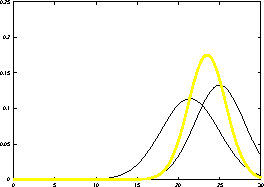
\includegraphics[width=0.3\columnwidth]{./images/kalman_filter_second_correction.pdf}
    }
    \end{figure}
   
\end{frame}

\begin{frame}
    \frametitle{Kalman Filter Assumptions}
    \note{Information taken from https://youtu.be/PiCC-SxWlH8}
    
    \begin{itemize}
    \item Noise and Gaussian Distributions
    \item Linear Motion and Observation Models
    \end{itemize}
    
    \begin{align*}
    \state_{t} &= A_{t} \state_{t-1} + B_{t}\controlCommand_{t} + \motionModelNoise_{t}\\
    \observation_{t} &= C_{t} \state_{t} + \measurementModelNoise_{t}
    \end{align*}
    \note{Kalman Filter requires that the noises be Gaussian and that the state result from a linear combination.}
    
    \centering
    \alert{What happens if these assumptions don't hold?}
    \note{Differential drive and Ackerman motion models are NOT linear models}
    \note{Observation models of a laser or a camera are not linear either.}
    \end{frame}
    
    \begin{frame}
    \frametitle{Non-linear Dynamical Systems}
    \note{Information taken from https://youtu.be/PiCC-SxWlH8}
    \begin{itemize}
    \item Real-life problems generally employ non-linear functions
    \end{itemize}
    
    % \begin{align*}
    % \state_{t} &= A_{t} \state_{t-1} + B_{t}\controlCommand_{t} + \motionModelNoise_{t}\\
    % \observation_{t} &= C_{t} \state_{t} + \measurementModelNoise_{t}
    % \end{align*}
    
    \begin{figure}[!h] 
    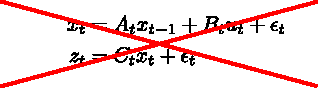
\includegraphics[width=0.4\columnwidth]{./images/kalman_filter_linear_equations_cross_out.pdf}
     \end{figure}
    
     \begin{align*}
     \state_{t} &= \motionModelFunction{\controlCommand_{t}, \state_{t-1}} + \motionModelNoise_{t}\\
     \observation_{t} &= \observationModelFunction{\state_{t}} + \measurementModelNoise_{t}
     \end{align*}
    
    \end{frame}
    
    \begin{frame}
     \frametitle{Linearity Assumption}
    
     \begin{figure}[!h]
     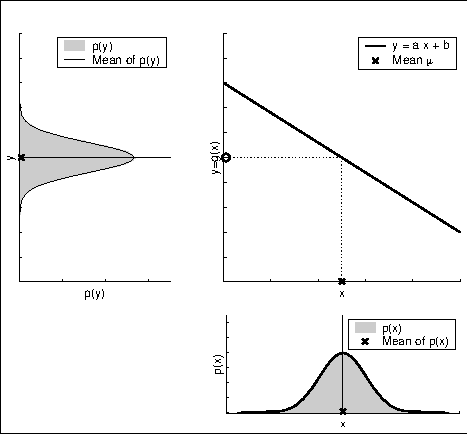
\includegraphics[width=0.5\columnwidth]{./images/linear_transformation_of_a_gaussian.pdf}
     \end{figure}
    \end{frame}
    
    \begin{frame}
    \frametitle{Nonlinear Function}
    
    \begin{figure}[!h]
    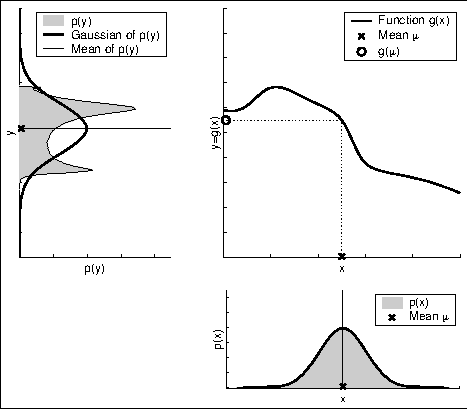
\includegraphics[width=0.5\columnwidth]{./images/nonlinear_transformation_of_a_gaussian.pdf}
    \end{figure}
    \end{frame}
    
    \begin{frame}
    \frametitle{Non-Gaussian Distributions}
    
    \note{Information taken from https://youtu.be/E-6paM\_Iwfc}
    
    \begin{itemize}
    \item Nonlinear functions lead to non-Gaussian distributions
    \item So, we can't apply the Kalman Filter!
    \end{itemize}
    
    \end{frame}
    
    \begin{frame}
     \frametitle{Linearization in EKF: First-order Taylor expansion}
    
     \note{Information taken from https://youtu.be/E-6paM\_Iwfc}
    
     \begin{itemize}
     \item Prediction:
     \begin{equation*}
     \motionModelFunction{\controlCommand_{t}, \state _{t-1}} \approx \motionModelFunction{\controlCommand_{t}, \mu _{t-1}} + \underbrace{\dfrac{\partial\motionModelFunction{\controlCommand_{t}, \mu _{t-1}}}{\partial\state _{t-1}}}_{\motionModelJacobian_{t}} (\state_{t-1} - \mu_{t-1})
     \end{equation*}
    
     \item Correction:
    
     \begin{equation*}
     \observationModelFunction{\state_{t}} \approx \observationModelFunction{\overline{\mu}_{t}} + \underbrace{\dfrac{\partial \observationModelFunction{\overline{\mu}_{t}}}{\partial \state_{t}}}_{\observationModelJacobian_{t}} (\state_{t} - \overline{\mu}_{t})
     \end{equation*}
    
     \end{itemize}
    
     $\motionModelJacobian_{t}$ and $\observationModelJacobian_{t}$ are called Jacobians.
    \end{frame}
    
    \begin{frame}
     \frametitle{Remembering Jacobians}
    
     \begin{itemize}
     \item In general it is a non-square matrix $m \times n$
     \item Given a vector function
    
     \begin{equation*}
     g(x) =
     \begin{bmatrix}
     g_{1}(x) \\
     g_{2}(x) \\
     \vdots \\
     gm(x)
     \end{bmatrix}
     \end{equation*}
    
     \item The Jacobian is defined as
     \begin{equation*}
     G_x =
     \begin{bmatrix}
     \dfrac{\partial g_{1}}{\partial x_{1}} & \dfrac{\partial g_{1}}{\partial x_{2}}& \dots & \dfrac{\partial g_{1}}{\partial x_{n}}\\
     \dfrac{\partial g_{2}}{\partial x_{1}} & \dfrac{\partial g_{2}}{\partial x_{2}}& \dots & \dfrac{\partial g_{2}}{\partial x_{n}}\\
     \vdots & \vdots& \vdots & \vdots\\
     \dfrac{\partial g_{m}}{\partial x_{1}} & \dfrac{\partial g_{m}}{\partial x_{2}}& \dots & \dfrac{\partial g_{m}}{\partial x_{n}}
     \end{bmatrix}
     \end{equation*}
     \end{itemize}
\end{frame}

\begin{frame}
    \frametitle{Remembering Jacobians}
    
    \begin{itemize}
    \item The Jacobian is the orientation of the tangent plane to a vector function at a given point
    \item The Jacobian is the generalization of the gradient of a scalar function
    \end{itemize}
    
    \begin{figure}[!h]
    \centering
    \subfloat[]
    {
    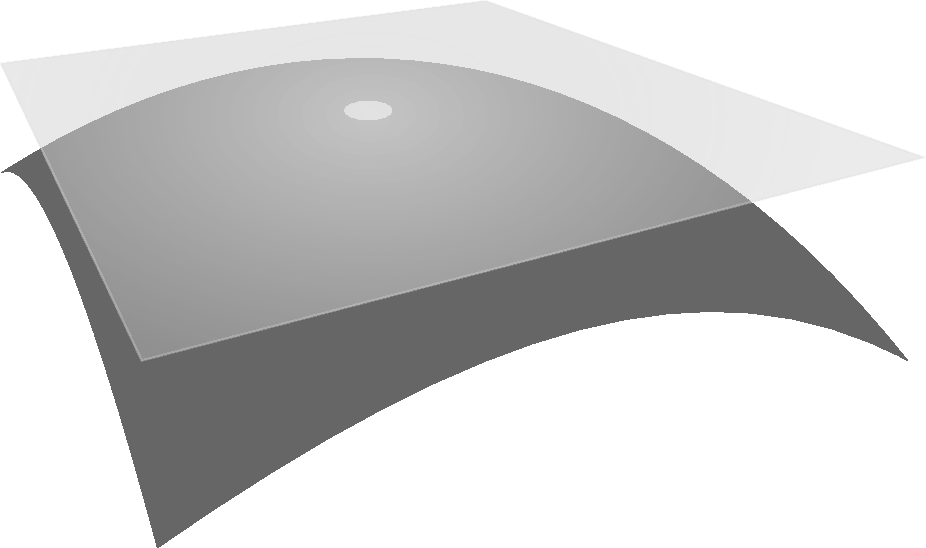
\includegraphics[valign=m,width=0.3\columnwidth]{./images/jacobian_tangent_plane.pdf}
    }
    \hspace{1cm} \subfloat[]
    {
    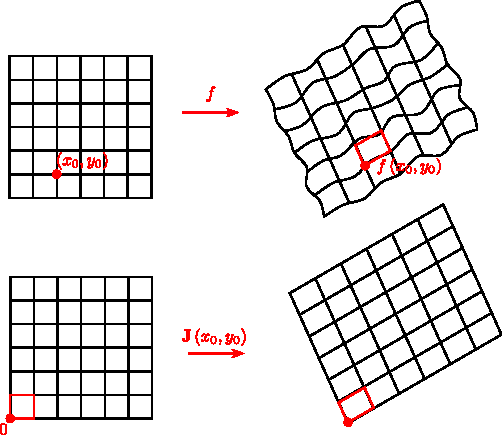
\includegraphics[valign=m,width=0.4\columnwidth]{./images/jacobian_local_linear_transform.pdf}
    }
    \end{figure}
    
    \begin{center}
    \end{center}
    
    \note{Info: https://angeloyeo.github.io/2020/07/24/Jacobian_en.html}
    
    \end{frame}
    
    
    \begin{frame}
     \frametitle{Linear Transformation}
    
     \begin{center}
     \movie[autostart,loop,poster]{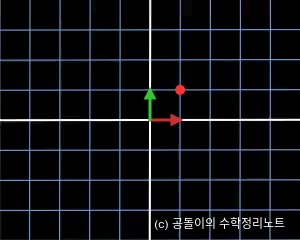
\includegraphics[width=0.6\columnwidth]{images/matrix_as_linear_transformation_video.jpg}}{videos/matrix_as_linear_transformation.mp4}
     \end{center}
    
     \note{Info: https://angeloyeo.github.io/2020/07/24/Jacobian_en.html}
    
    \end{frame}
    
    
    \begin{frame}
     \frametitle{Non-Linear Transformation}
    
     \begin{center}
     \movie[autostart,loop,poster]{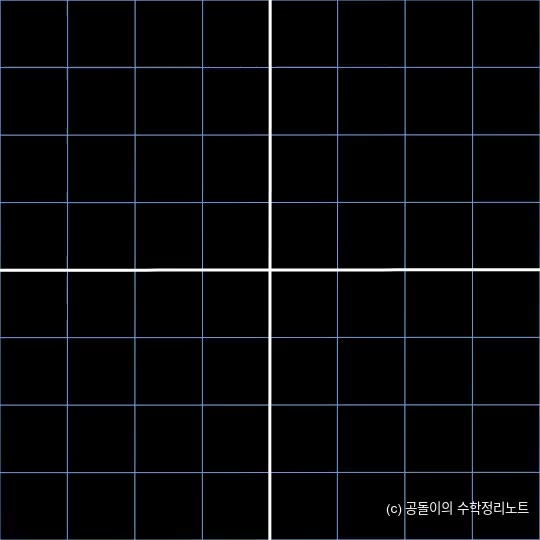
\includegraphics[width=0.5\columnwidth]{images/jacobian_nonlinear_transform_video.jpg}}{videos/jacobian_nonlinear_transform.mp4}
     \end{center}
    
     \note{Info: https://angeloyeo.github.io/2020/07/24/Jacobian_en.html}
    
    \end{frame}
    
    \begin{frame}
     \frametitle{Non-Linear (but Locally Linear) Transformation}
    
     \begin{center}
     \movie[autostart,loop,poster]{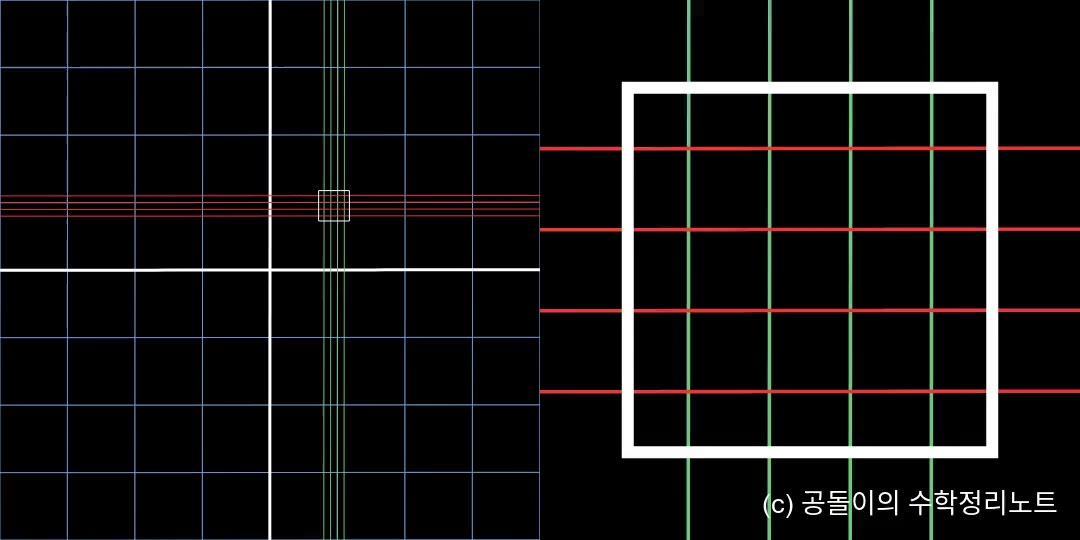
\includegraphics[width=\columnwidth]{images/jacobian_locally_linear_video.jpg}}{videos/jacobian_locally_linear.mp4}
     \end{center}
    
     \note{Info: https://angeloyeo.github.io/2020/07/24/Jacobian_en.html}
    
    \end{frame}
    
    
    \begin{frame}
     \frametitle{Linearization in EKF}
    
     \begin{figure}[!h]
     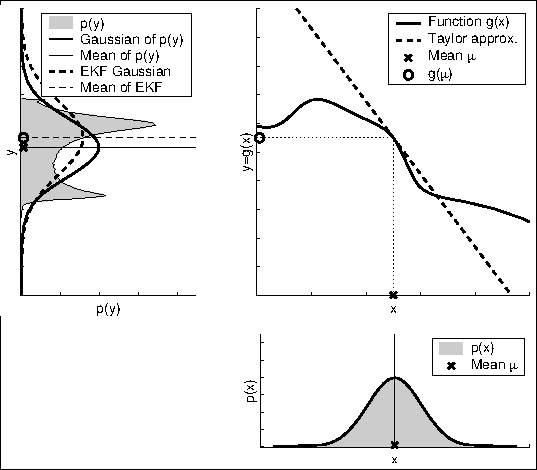
\includegraphics[width=0.5\columnwidth]{./images/linearization_applied_by_ekf.pdf}
     \end{figure}
    \end{frame}
    
    
    \begin{frame}
     \frametitle{Quality of Linearization in EKF}
    
     \begin{figure}[!h]
     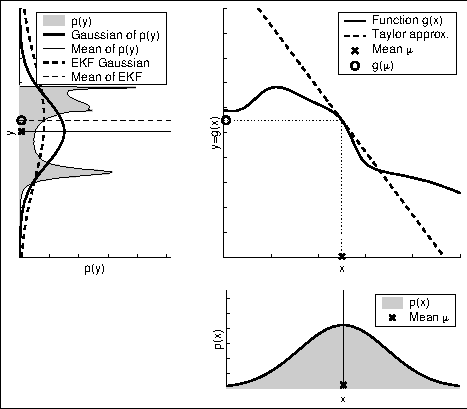
\includegraphics[width=0.5\columnwidth]{./images/dependency_approximation_quality_spread.pdf}
     \end{figure}
    \end{frame}
    
    \begin{frame}
     \frametitle{Quality of Linearization in EKF}
    
     \begin{figure}[!h]
    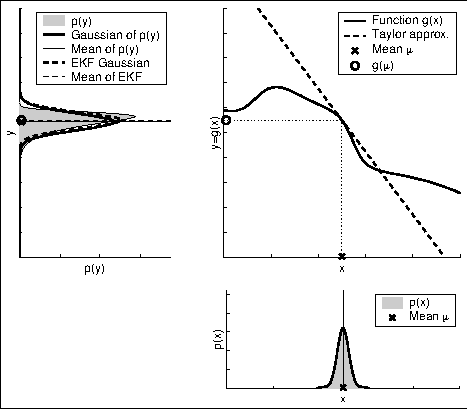
\includegraphics[width=0.5\columnwidth]{./images/dependency_approximation_quality_narrow.pdf}
    \end{figure}
    \end{frame}
    
    \begin{frame}
    \frametitle{Linearized Motion Model}
    \note{Information taken from https://youtu.be/PiCC-SxWlH8}
    
    \begin{itemize}
    \item Linearizing the model is given by:
    \begin{align*}
    p(\state_{t} | \controlCommand_{t}, \state _{t-1}) &\approx \det(2 \pi \motionParametersCovariance_{t})^{\frac{1}{2}}\\
     &\exp (-\dfrac{1}{2} (\state_{t} - \motionModelFunction{\controlCommand_{t}-\mu_{t-1}} - \motionModelJacobian_{t}(\state_{t-1}-\mu_{t-1}))^{\top}\\
     &\inverse{\motionParametersCovariance_{t}} (\state_{t} - \underbrace{\motionModelFunction{\controlCommand_{t},\mu_{t-1}} - \motionModelJacobian_{t} (\state_{t-1}-\mu_{t-1})}_{\text{model linearized}}))
    \end{align*}
    
    \item $\motionParametersCovariance_{t}$ describes motion noise
    \end{itemize}
    \end{frame}
    
    \begin{frame}
    \frametitle{Linearized observation model}
    \note{Information taken from https://youtu.be/PiCC-SxWlH8}
    
    \begin{itemize}
    \item Linearizing the model is given by:
    \begin{align*}
    p(\observation_{t} | \state_{t}) &\approx \det(2 \pi \observationModelCovariance_{t})^{\frac{1}{2}}\\
    &\exp (-\dfrac{1}{2} (\observation_{t} - \observationModelFunction{\overline{\mu_{t}}} - \observationModelJacobian_{t}(\state_{t} - \overline{\mu _{t}}))^{\top}\\
     &\inverse{\observationModelCovariance_{t}} (\observation_{t} - \underbrace{\observationModelFunction{\overline{\mu_{t}}} - \observationModelJacobian_{t} (\state_{t}-\overline{\mu_{t}})}_{\text{linearized model}}))
     \end{align*}
    
     \item $\observationModelCovariance_{t}$ describes the measurement noise
     \end{itemize}
    
    
\end{frame}

\begin{frame}
    \frametitle{Extended Kalman Filter Algorithm}
    \note{information taken from https://youtu.be/PiCC-SxWlH8}
   
    \begin{algorithmic}[1]
    \Procedure{ExtendedKalmanFilter}{$\mu_{t-1}, \covariance_{t-1}, \controlCommand_{t}, \observation_{t}$}
    \State $\overline{\mu}_{t} = \motionModelFunction{\controlCommand_{t}, \mu_{t-1}}$
    \State $\overline{\covariance}_{t} = \motionModelJacobian_{t} \covariance_{t-1} \motionModelJacobian_{t}^{\top}+\motionParametersCovariance_{t}$
    \Statex
    \State $\kalmanGain_{t} = \overline{\covariance}_{t} \observationModelJacobian_{t}^{\top} (\observationModelJacobian_{t} \overline{\covariance}_{t} \observationModelJacobian_{t} + \observationModelCovariance_{t})^{-1} $
    \State $\mu_{t} = \overline{\mu}_{t} + \kalmanGain_{t} (\observation_{t} - \observationModelFunction{\overline{\mu}_{t}})$
    \State $\covariance_{t} = (I - \kalmanGain_{t} \observationModelJacobian_{t}) \overline{\covariance}_{t}$
    \State \Return $\mu_{t}, \covariance_{t}$
    \EndProcedure
    \end{algorithmic}
   \end{frame}
   
   \section{EKF Location for feature-based map}
   
   \begin{frame}
    \frametitle{Odometry as controls}
    \note{information taken from https://youtu.be/PiCC-SxWlH8}
   
    \begin{figure}[!h]
    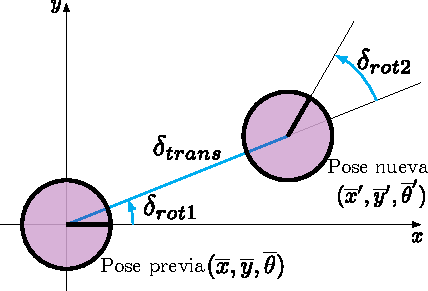
\includegraphics[width=0.6\columnwidth]{./images/odometry_as_controls.pdf}
    \end{figure}
   
    \begin{equation*}
    \controlCommand = (\delta _{rot1}, \delta _{trans}, \delta _{rot2})
    \end{equation*}
   
   \end{frame}
   
   \begin{frame}
    \frametitle{Motion model}
    \note{information taken from https://youtu.be/PiCC-SxWlH8}
   
    \begin{itemize}
    \item Motion Model Odometry
    \begin{equation*}
    \begin{bmatrix}
    x^{\prime} \\
    y^{\prime} \\
    \theta^{\prime}
    \end{bmatrix} =
    \underbrace{
    \begin{bmatrix}
    x \\
    and \\
    \theta
    \end{bmatrix} +
    \begin{bmatrix}
    \delta_{trans}\cos(\theta+\delta_{rot_{1}}) \\
    \delta_{trans}\sin(\theta+\delta_{rot_{1}}) \\
    \delta_{rot_{1}} + \delta_{rot_{2}}
    \end{bmatrix}
    }_{\motionModelFunction{\controlCommand_{t}, \state_{t-1}}} + \normalDistribution{0}{\motionParametersCovariance_{t}}
    \end{equation*}
    \item Linearization
    \begin{equation*}
    \motionModelFunction{\controlCommand_{t}, \state _{t-1}} \approx \motionModelFunction{\controlCommand_{t}, \mu _{t-1}} + \motionModelJacobian_{t}(\state _{t-1}-\mu _{t-1})
    \end{equation*}
    \end{itemize}
   
   \end{frame}
   
   \begin{frame}
    \frametitle{Jacobians of the motion model}
    \note{information taken from https://youtu.be/PiCC-SxWlH8}
    We calculate the Jacobian with respect to the state
    \begin{equation*}
    \motionModelJacobian_{t} = \dfrac{\delta\motionModelFunction{\controlCommand_{t},\mu _{t-1}}}{\delta \state _{t-1}} =
    \begin{bmatrix}
    \dfrac{\delta x^{\prime}}{\delta \mu _{t-1,x}} & \dfrac{\delta x^{\prime}}{\delta \mu _{t-1,y}} & \dfrac{\delta x^{\prime}}{\delta \mu _{t-1,\theta}}\\
    \dfrac{\delta y^{\prime}}{\delta \mu _{t-1,x}} & \dfrac{\delta y^{\prime}}{\delta \mu _{t-1,y}} & \dfrac{\delta y^{\prime}}{\delta \mu _{t-1,\theta}}\\
    \dfrac{\delta \theta^{\prime}}{\delta \mu _{t-1,x}} & \dfrac{\delta \theta^{\prime}}{\delta \mu _{t-1,y}} & \dfrac{\delta \theta^{\prime}}{\delta \mu _{t-1,\theta}}\\
    \end{bmatrix}
    \end{equation*}
   
    \begin{equation*}
    \motionModelJacobian_{t} =
    \begin{bmatrix}
    1 & 0 & -\delta_{trans} \sin(\theta + \delta_{rot_{1}})\\
    0 & 1 & \delta_{trans} \cos(\theta + \delta_{rot_{1}})\\
    0 & 0 & 1\\
    \end{bmatrix}
    \end{equation*}
\end{frame}

\begin{frame}
    \frametitle{Jacobians of the motion model}
    \note{information taken from https://youtu.be/PiCC-SxWlH8}
    
    We calculate the Jacobian with respect to the control command
    \begin{equation*}
    \motionModelJacobianControl{t} = \dfrac{\delta\motionModelFunction{\controlCommand_{t},\mu_{t-1}}}{\delta \controlCommand_{t}} =
    \begin{bmatrix}
    \dfrac{\delta x^{\prime}}{\delta \controlCommand_{t,\delta_{rot_{1}}}} & \dfrac{\delta x^{\prime}}{\delta \controlCommand_{t,\delta_{trans}}} & \dfrac{\delta x^{\prime}}{\delta \controlCommand_{t,\delta_{rot_{2}}}}\\
     \dfrac{\delta y^{\prime}}{\delta \controlCommand_{t,\delta _{rot_{1}}}} & \dfrac{\delta y^{\prime}}{\delta \controlCommand_{t,\delta _{trans}}} & \dfrac{\delta y^{\prime}}{\delta \controlCommand_{t,\delta _{rot_{2}}}}\\
     \dfrac{\delta \theta^{\prime}}{\delta \controlCommand_{t,\delta _{rot_{1}}}} & \dfrac{\delta \theta^{\prime}}{\delta \controlCommand_{t,\delta _{trans}}} & \dfrac{\delta \theta^{\prime}}{\delta \controlCommand_{t,\delta _{rot_{2}}}}
     \end{bmatrix}
     \end{equation*}
    
     \begin{equation*}
     \motionModelJacobianControl_{t} =
     \begin{bmatrix}
     -\delta_{trans} \sin(\theta + \delta _{rot_{1}}) & \cos(\theta + \delta _{rot_{1}}) & 0\\
     \delta _{trans} \cos(\theta + \delta _{rot_{1}}) & \sin(\theta + \delta _{rot _{1}}) & 0\\
     1 & 0 & 1\\
     \end{bmatrix}
     \end{equation*}
    \end{frame}
    
    \begin{frame}
     \frametitle{Observation model}
     \note{information taken from https://youtu.be/PiCC-SxWlH8}
     \begin{itemize}
     \item Range-bearing model
     \begin{equation*}
     \observation_{t}^{i} =
     \begin{bmatrix}
     r_{t}^{i}\\
     \phi_{t}^{i}
     \end{bmatrix} =
     \begin{bmatrix}
     \sqrt{(m_{j,x}-x)^{2} + (m_{j,y}-y)^{2}}\\
     \atantwo(m_{j,y}-y, m_{j,x}-x) -\theta
     \end{bmatrix}
     + \normalDistribution{0}{\observationModelCovariance_{t}}
     \end{equation*}
    
     \item Linearization
     \begin{equation*}
     \observationModelFunction{\state_{t}, m} \approx \observationModelFunction{\overline{\mu}_{t}} + \observationModelJacobian_{t}^{i}(\state_{t}-\overline{\mu}_{t})
     \end{equation*}
     \end{itemize}
    
    \end{frame}
    
    \begin{frame}
     \frametitle{Jacobians of the observation model}
     \note{information taken from https://youtu.be/PiCC-SxWlH8}
     We calculate the Jacobian with respect to the state
     \begin{equation*}
     \observationModelJacobian_{t} = \dfrac{\delta\observationModelFunction{\overline{\mu}_{t},m}}{\delta \state_{t}} =
     \begin{bmatrix}
     \dfrac{\delta r_{t}^{i}}{\delta \overline{\mu}_{t,x}} & \dfrac{\delta r_{t}^{i}}{\delta \overline{\mu}_{t,y}} & \dfrac{\delta r_{t}^{i}}{\delta \overline{\mu}_{t,\theta}}\\
     \dfrac{\delta \phi _{t}^{i}}{\delta \overline{\mu}_{t,x}} & \dfrac{\delta \phi _{t}^{i}}{\delta \overline{\mu}_{t,y}} & \dfrac{\delta \phi _{t}^{i}}{\delta \overline{\mu}_{t,\theta}}
     \end{bmatrix}
     \end{equation*}
    
     \begin{equation*}
     \observationModelJacobian_{t}^{i} =
     \begin{bmatrix}
     -\dfrac{m_{j,x} - \overline{\mu}_{t,x}}{\sqrt{q}} & -\dfrac{m_{j,y} - \overline{\mu}_{t,y}}{\sqrt{q}} & 0\\
     \dfrac{m_{j,y} - \overline{\mu}_{t,y}}{q} & -\dfrac{m_{j,x} - \overline{\mu}_{t,x}}{q} & -1
     \end{bmatrix}
     \end{equation*}
     where
     \begin{equation*}
     q = (m_{j,x}-\overline{\mu}_{t,x})^{2} + (m_{j,y}-\overline{\mu}_{t,y})^{2}
     \end{equation*}
\end{frame}

\begin{frame}
    \frametitle{Extended Kalman Filter Algorithm}
    \note{information taken from https://youtu.be/PiCC-SxWlH8}
    \footnotesize
    \begin{algorithmic}[1]
    \State ExtendedKalmanFilter({$\mu_{t-1}, \covariance_{t-1}, \controlCommand_{t}, \observation_{t}$, $c_{t}$, $m$})
    \State $\theta = \mu_{t-1,\theta}$
   
    \State $
    \motionModelJacobian_{t} =
    \begin{bmatrix}
    1 & 0 & -\delta_{trans} \sin(\theta + \delta_{rot_{1}})\\
    0 & 1 & \delta_{trans} \cos(\theta + \delta_{rot_{1}})\\
    0 & 0 & 1\\
    \end{bmatrix}
    $
    \State $
    \motionModelJacobianControl_{t} =
    \begin{bmatrix}
    -\delta_{trans} \sin(\theta + \delta _{rot_{1}}) & \cos(\theta + \delta _{rot_{1}}) & 0\\
    \delta _{trans} \cos(\theta + \delta _{rot_{1}}) & \sin(\theta + \delta _{rot _{1}}) & 0\\
    1 & 0 & 1\\
    \end{bmatrix}
    $
    \State $
    \motionModelCovariance_{t} =
    \begin{bmatrix}
    \alpha_{1}\delta^{2}_{rot_{1}} + \alpha_{2}\delta^{2}_{trans} & 0 & 0\\
    0 & \alpha_{3} \delta^{2}_{trans} + \alpha_{4} \left( \delta^{2}_{rot_{1}} + \delta^{2}_{rot_{2}} \right) & 0\\
    0 & 0 & \alpha_{1}\delta^{2}_{rot_{2}} + \alpha_{2}\delta^{2}_{trans}\\
    \end{bmatrix}
    $
    \State $\overline{\mu}_{t} = \mu_{t-1} +
    \begin{bmatrix}
    \delta_{trans}\cos(\theta+\delta_{rot_{1}}) \\
    \delta_{trans}\sin(\theta+\delta_{rot_{1}}) \\
    \delta_{rot_{1}} + \delta_{rot_{2}}
    \end{bmatrix}$
    \State $\overline{\covariance}_{t} = \motionModelJacobian_{t} \covariance_{t-1} \motionModelJacobian_{t}^{\top}+\motionModelJacobianControl_{t} \motionModelCovariance_{t} \motionModelJacobianControl_{t}^{\top}$
    \end{algorithmic}
    \vspace{1em}
    $M_{t}$ is a covariance that models the noise in the control commands.
    $\motionModelJacobianControl_{t} \motionModelCovariance_{t} \motionModelJacobianControl_{t}^{\top}$ refers to the uncertainty that is added due to noise in the control commands.
   
   \end{frame}
   
   \begin{frame}
   \frametitle{Prediction step}
   \note{Information taken from https://youtu.be/PiCC-SxWlH8}
   
   \begin{figure}[!h]
   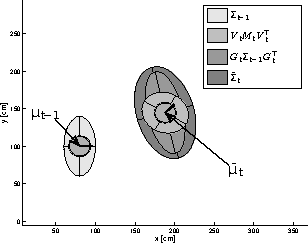
\includegraphics[width=0.5\columnwidth]{./images/ekf_prediction_step.pdf}
   \caption{Pose Prediction}
   \end{figure}
   
   \end{frame}
   
   \begin{frame}
   \frametitle{Extended Kalman Filter Algorithm}
   \note{Information taken from https://youtu.be/PiCC-SxWlH8}
   \footnotesize
   \begin{algorithmic}[1]
   \State
   $ \observationModelCovariance_{t} =
   \begin{bmatrix}
   \sigma_{r}^{2} & 0\\
   0 & \sigma_{\phi}^{2}
    \end{bmatrix}
    $
    \For {all observed features $z_{t}^{i} = (r_{t}^{i}, \phi_{t}^{i})^{\top}$}
   
    \State $ j = c_{t}^{i}$
    \State $ q = (m_{j,x}-\overline{\mu}_{t,x})^{2} + (m_{j,y}-\overline{\mu}_{t,y})^{2} $
    \State
    $ \hat{\observation}_{t}^{i} =
    \begin{bmatrix}
    \sqrt{q}\\
    \atantwo(m_{j,y}-\overline{\mu}_{t,y}, m_{j,x}-\overline{\mu}_{t,x}) - \overline{\mu}_{t,\theta}
    \end{bmatrix}
    $
    \State
    $ \observationModelJacobian_{t}^{i} =
    \begin{bmatrix}
    -\dfrac{m_{j,x} - \overline{\mu}_{t,x}}{\sqrt{q}} & -\dfrac{m_{j,y} - \overline{\mu}_{t,y}}{\sqrt{q}} & 0\\
    \dfrac{m_{j,y} - \overline{\mu}_{t,y}}{q} & -\dfrac{m_{j,x} - \overline{\mu}_{t,x}}{q} & -1
    \end{bmatrix}
    $
   
    \State $S_{t}^{i} = \observationModelJacobian_{t}^{i} \overline{\covariance}_{t} \observationModelJacobian_{t}^{i^{\top}} + \observationModelCovariance_{t} $
   
    \State $\kalmanGain_{t}^{i} = \overline{\covariance}_{t} {\observationModelJacobian_{t}^{i}}^{\top} S_{t}^{i^{-1}} $
    \State $\overline{\mu}_{t} = \overline{\mu}_{t} + \kalmanGain_{t}^{i}(\observation_{t} - \hat{\observation}_{t}^{i})$
    \State $\overline{\covariance}_{t} = (I - \kalmanGain_{t}^{i}\observationModelJacobian_{t}^{i})\overline{\covariance}_{t}$
   
    \EndFor
    \State $\mu_{t} = \overline{\mu}_{t}$
    \State $\covariance_{t} = \overline{\covariance}_{t}$
   
    \State \Return $\mu_{t}, \covariance_{t}$
    \end{algorithmic}
   
   
\end{frame}

\begin{frame}
    \frametitle{Measurement Prediction}
    \note{information taken from https://youtu.be/PiCC-SxWlH8}
    
    \begin{figure}[!h]
    \centering
    \subfloat[Pose Prediction]
    {
    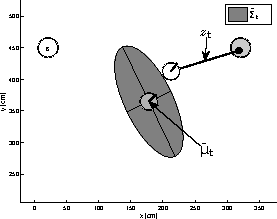
\includegraphics[width=0.45\columnwidth]{./images/ekf_pose_prediction.pdf}
    }
    \subfloat[Measurement Prediction]
    {
    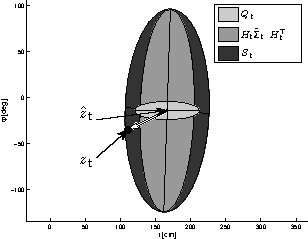
\includegraphics[width=0.45\columnwidth]{./images/ekf_measurement_prediction.pdf}
    }
    \end{figure}
    \footnotesize
    \begin{itemize}
    \item The robot's ground truth and the measurement are indicated by the white circle and the bold line, respectively.
    
    \item The white arrow indicates the \textbf{innovation} difference between observation and prediction of measurement. \end{itemize}
    
    \end{frame}
    
    \begin{frame}
    \frametitle{Correction step}
    \note{Information taken from https://youtu.be/PiCC-SxWlH8}
    
    \begin{figure}[!h]
    \centering
    \subfloat[Measurement Prediction]
    {
    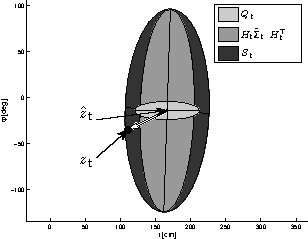
\includegraphics[width=0.45\columnwidth]{./images/ekf_measurement_prediction.pdf}
    }
    \subfloat[Measurement Correction]
    {
    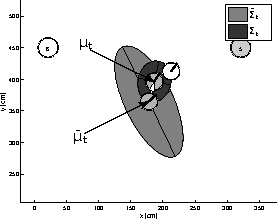
\includegraphics[width=0.45\columnwidth]{./images/ekf_measurement_correction.pdf}
    }
    \end{figure}
    
    \end{frame}
    
    \begin{frame}
    \frametitle{Example: EKF Localization 2D}
    \note{Information taken from the book Probabilistic Robotics}
    
    \begin{figure}[!h]
    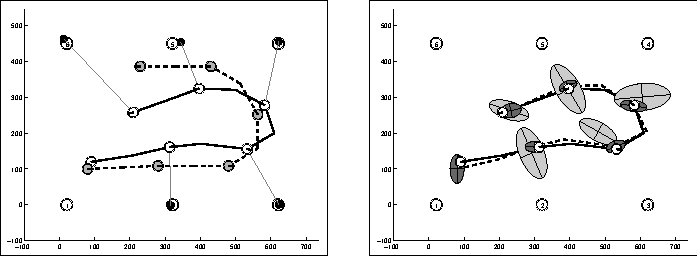
\includegraphics[width=\columnwidth]{./images/ekf_localization_example.pdf}
    \end{figure}
    
    The solid line is the ground truth. In the first graph, the dotted line is the odometry, and in the second graph, it is the estimate given by the EKF.
    
    \end{frame}
    
    \begin{frame}
    \frametitle{EKF Summary}
    \note{Information taken from https://youtu.be/PiCC-SxWlH8}
    
    \begin{itemize}
    \item It is an extension of the Kalman Filter
    \item A way to work with nonlinearities
    \item Performs local linearizations
    \item Works well in practice for moderately nonlinear cases
    \item Large uncertainties lead to increased error
    \end{itemize}
    
    \end{frame}
    
    \begin{frame}
    \frametitle{Extended Kalman Filter}
    
    \note{Information taken from:
    Cyrill Stachniss KF and EKF: https://youtu.be/E-6paM_Iwfc
    Chebrolu EKF Localization: https://youtu.be/PiCC-SxWlH8}
    
    \footnotesize 
    \url{https://automaticaddison.com/extended-kalman-filter-ekf-with-python-code-example/}
     \url{https://github.com/shangzhouye/EKF-SLAM-on-Turtlebot3}
    
     \url{https://github.com/ser94mor/sensor-fusion}
    
     \url{https://github.com/AtsushiSakai/PythonRobotics}
    
     It may be that the tp is just in python and the final tp is in ROS2.
    
     \url{https://github.com/debbynirwan/mcl}
    
    
\end{frame}
